\chapter{Защита страниц}
\label{protection}

На страницы Викиданных устанавливается защита для предотвращения повторяющегося вандализма или спама. 

\begin{marginfigure}[5.0cm]
{
	\setlength{\fboxsep}{0pt}%
	\setlength{\fboxrule}{1pt}%
	{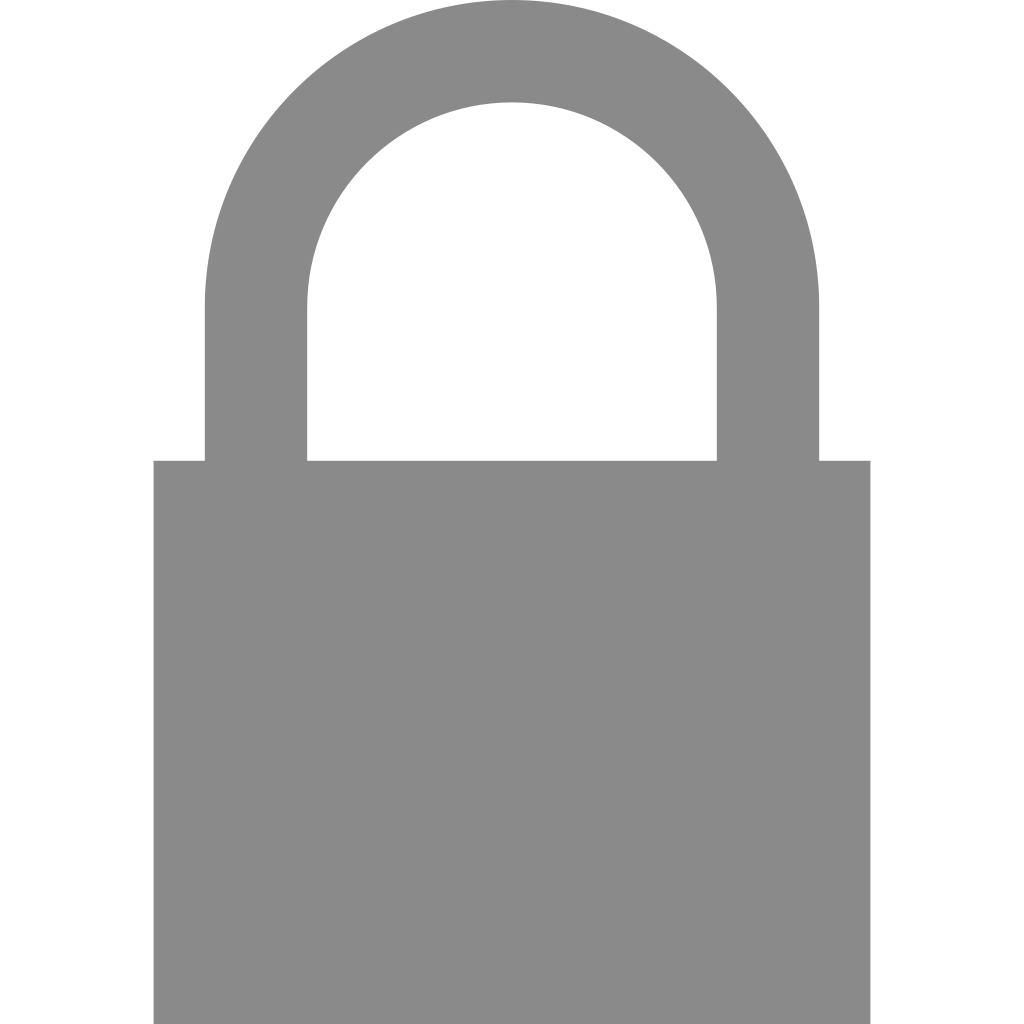
\includegraphics[width=0.3\linewidth]{"chapter/oblast_of_Russia/Semi_protect.png"}}
}
\caption [Иконка. Частичная защита или полузащита.]{Частичная защита или полузащита.}%
\label{fig:legend_population}%
\end{marginfigure}

\begin{marginfigure}[0.0cm]
{
	\setlength{\fboxsep}{0pt}%
	\setlength{\fboxrule}{1pt}%
	{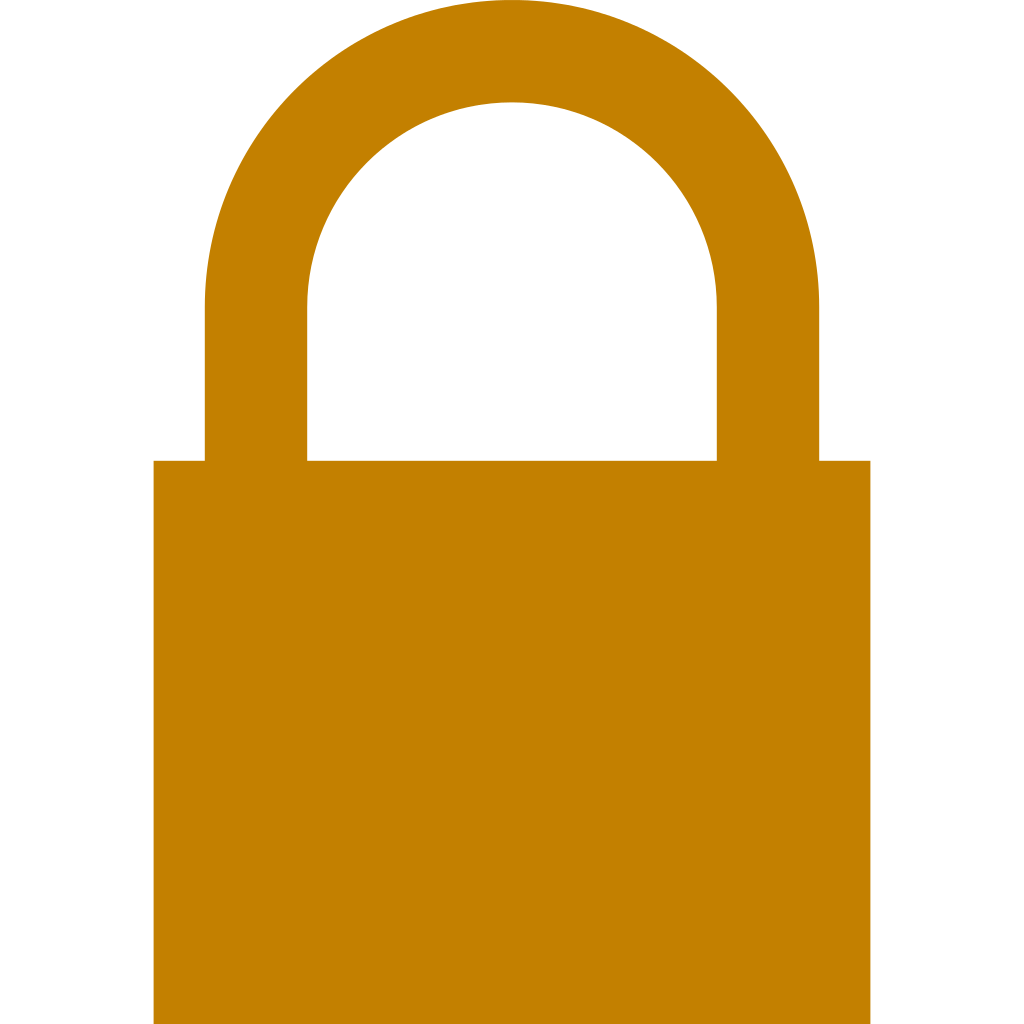
\includegraphics[width=0.3\linewidth]{"chapter/oblast_of_Russia/Full_protect.png"}}
	{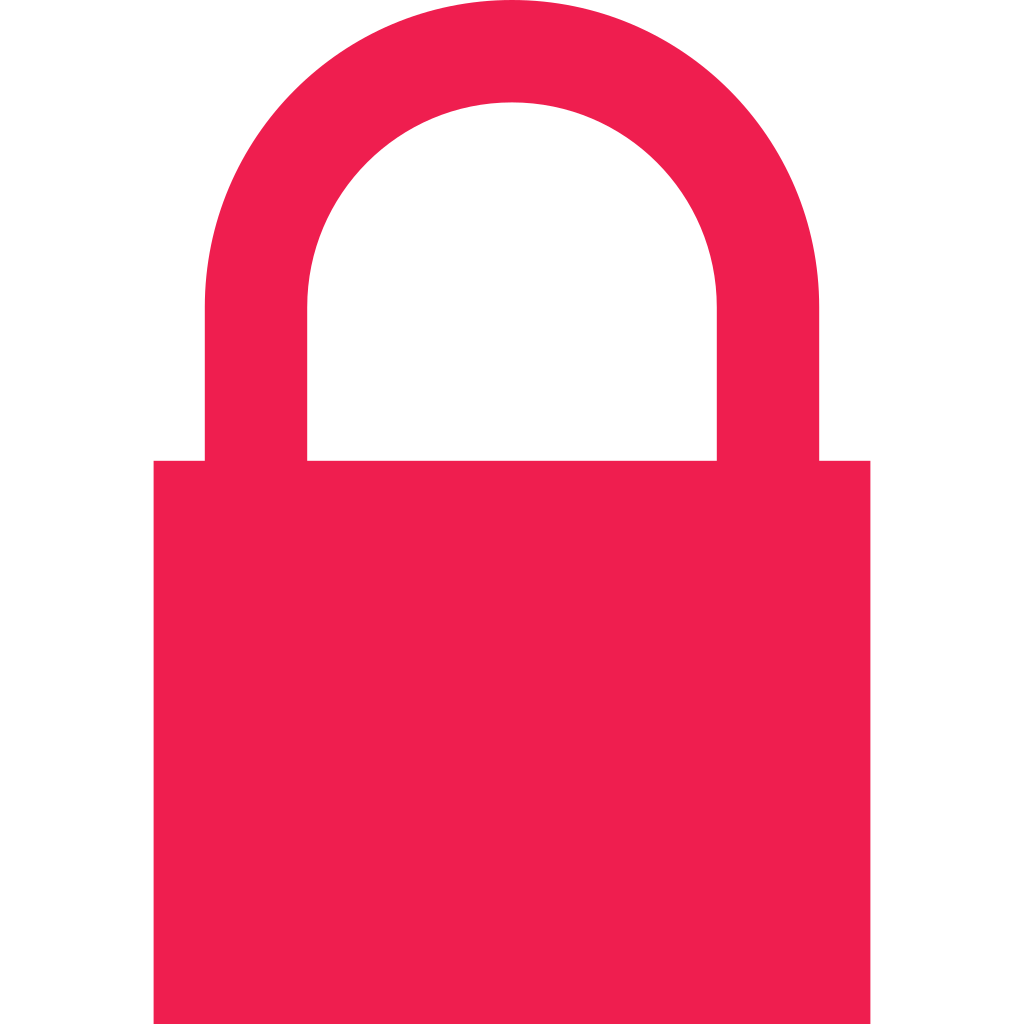
\includegraphics[width=0.3\linewidth]{"chapter/oblast_of_Russia/Permanent_protect.png"}}
}
\caption [Иконка. Полная защита.]{Полная защита..}%
\label{fig:legend_population}%
\end{marginfigure}

\begin{marginfigure}[0.0cm]
{
	\setlength{\fboxsep}{0pt}%
	\setlength{\fboxrule}{1pt}%
	{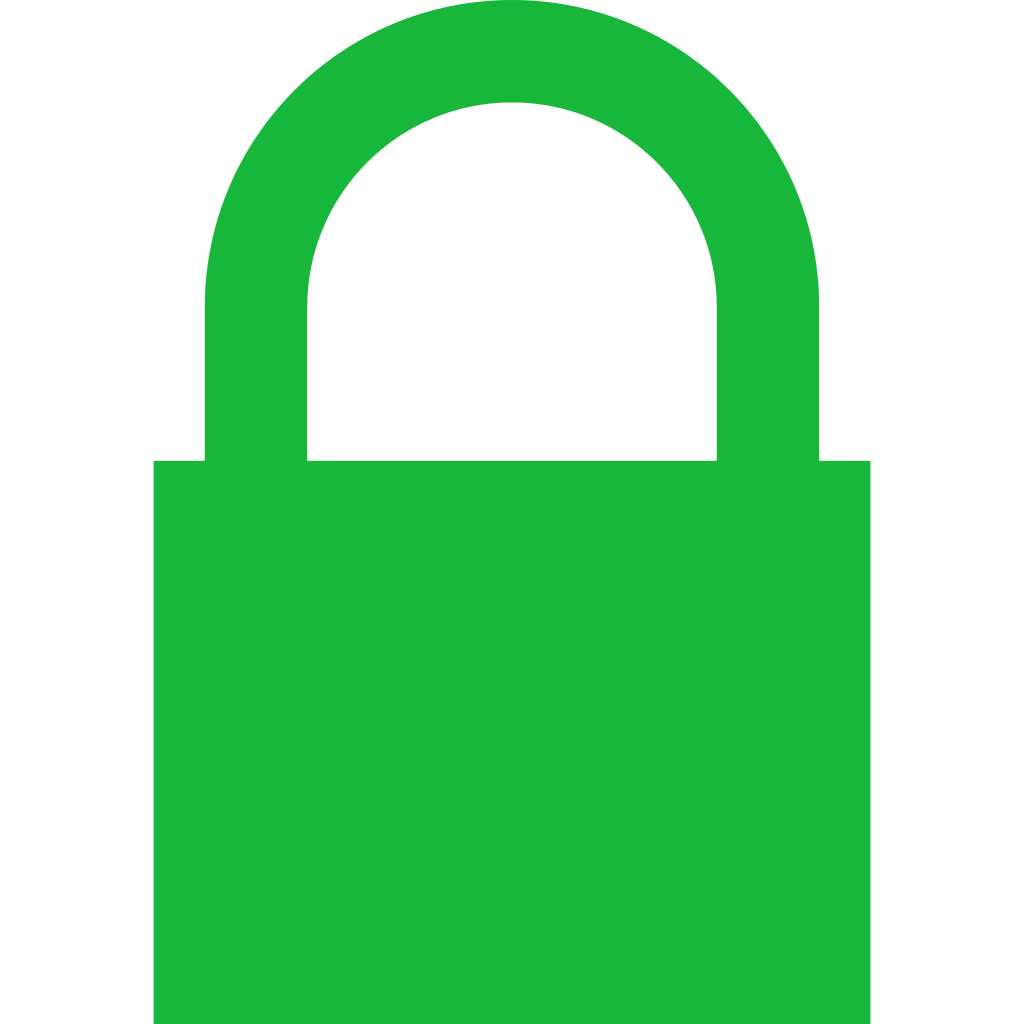
\includegraphics[width=0.3\linewidth]{"chapter/oblast_of_Russia/Move_protect.png"}}
}
\caption [Иконка. Защита от переименования.]{Защита от переименования.}%
\label{fig:legend_population}%
\end{marginfigure}

Существует несколько видов защиты:
\begin{itemize}
  \item Частичная защита или полузащита (обозначается серым замком) разрешает редактировать страницу только автоподтверждённым/подтверждённым участникам.
  \item Полная защита (обозначается оранжевым или красным замком) ограничивает круг редакторов администраторами.
  \item Защита от переименования (обозначается зелёным замком) не ограничивает возможность редактировать страницу, однако переименовать её могут только администраторы. Большинство популярных страниц защищено от переименования. Защита от переименования не может быть применена к страницам элементов или свойств.
  \item Защита от создания (как полная, так и частичная защита обозначается синим замком) может применяться к удалённым или несуществующим страницам. Однако, как и защита от переименования, она не может применяться к удалённым элементам или свойствам.
  \begin{itemize}
	\item При полной защите от создания страницу не может создать никто, кроме администраторов.
	\item При частичной защите от создания страницу могут создать также автоподтверждённые и подтверждённые участники.
  \end{itemize}
\end{itemize}

\begin{marginfigure}[0.0cm]
{
	\setlength{\fboxsep}{0pt}%
	\setlength{\fboxrule}{1pt}%
	{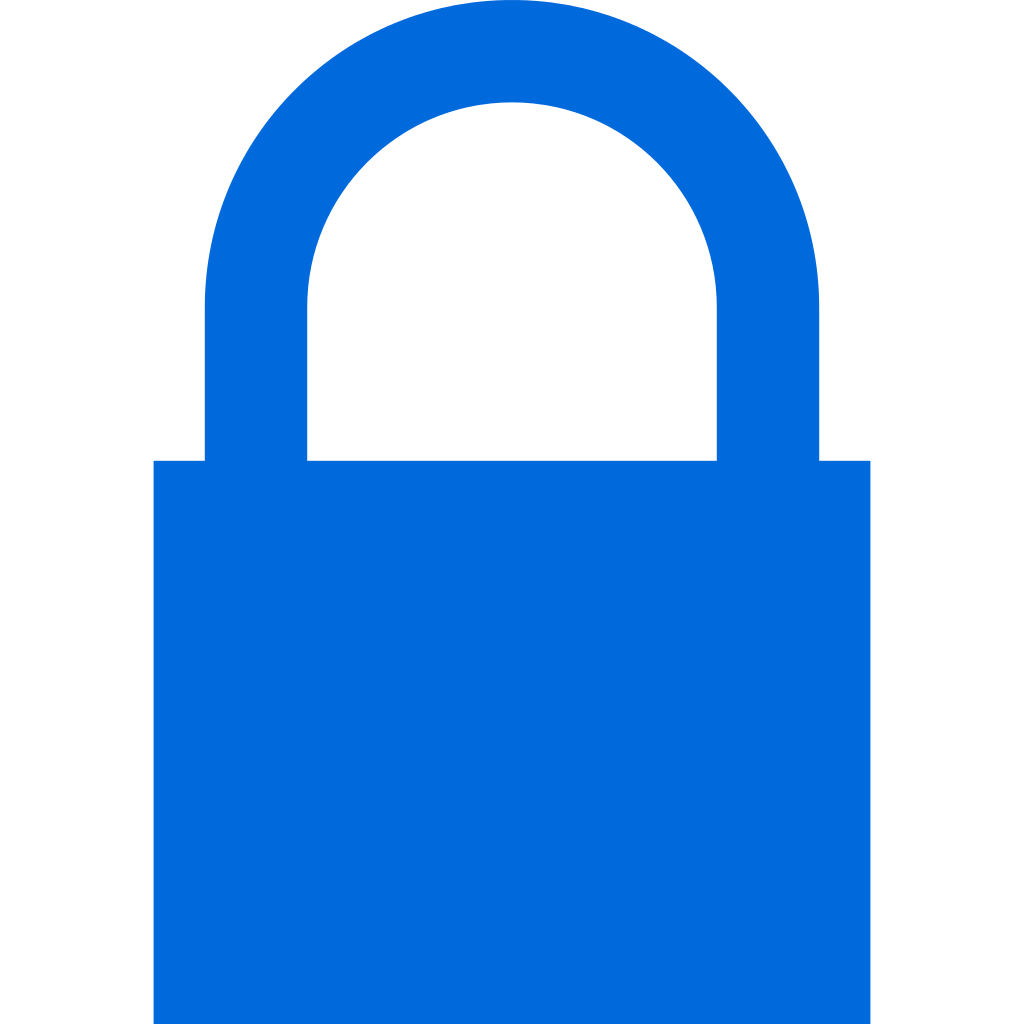
\includegraphics[width=0.3\linewidth]{"chapter/oblast_of_Russia/Create_protect.png"}}
}
\caption [Иконка. Защита от создания.]{Защита от создания.}%
\label{fig:legend_population}%
\end{marginfigure}

\begin{marginfigure}[0.0cm]
{
	\setlength{\fboxsep}{0pt}%
	\setlength{\fboxrule}{1pt}%
	{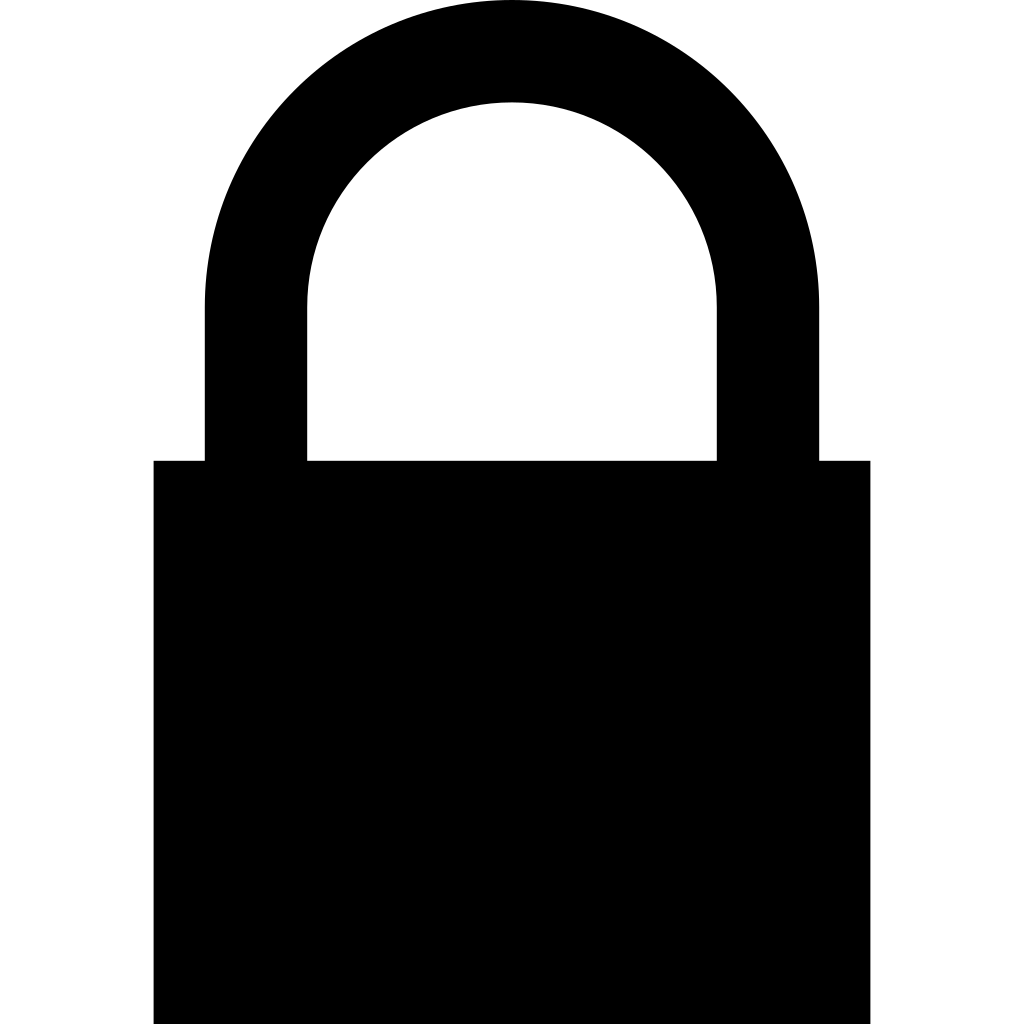
\includegraphics[width=0.3\linewidth]{"chapter/oblast_of_Russia/Office_action.png"}}
}
\caption [Иконка. Официальное действие.]{Официальное действие.}%
\label{fig:legend_population}%
\end{marginfigure}

В крайне редких случаях Фонд Викимедиа может защитить страницу в качестве официального действия (\textit{office action}, обозначается чёрным замком). Официальные действия совершаются только в результате формальной вневикипедийной жалобы, всегда публично объявляются и выполняются только сотрудниками Фонда Викимедиа или членами Совета попечителей.

Документация Викиданных содержит дополнительные материалы о защите страниц\protect\footnotemark
\footnotetext{См. правила защиты страниц \href{https://goo-gl.me/OkHtF}{https://goo-gl.me/OkHtF}.}.
